\section{Subgradient and subdifferential}


\subsection{Problem № 1} 
Find $\partial f(x)$, if $f(x) = $ \textbf{Leaky ReLU}$(x) = $ $\begin{cases}
   x, if x > 0 \\
   0.01x , otherwise
 \end{cases}$
 
\underline{\textbf{Solution:}}
By Dubovitsky-Milutin theorem we can get:
\begin{equation*}
    \partial f(x) = \begin{cases}
        1, x > 0 \\
        [0.01; 1], x = 0 \\
        0.01, x < 0 
    \end{cases}
\end{equation*}

\underline{\textbf{Answer:}}
$
    \partial f(x) = \begin{cases}
        1, x > 0 \\
        [0.01; 1], x = 0 \\
        0.01, x < 0 
    \end{cases}
$
\subsection{Problem №2}
Find subdifferential of a function $f(x) = cosx$ on the set $X = [0, \frac{3}{2} \pi ]$.

\underline{\textbf{Solution:}}
\begin{center}
    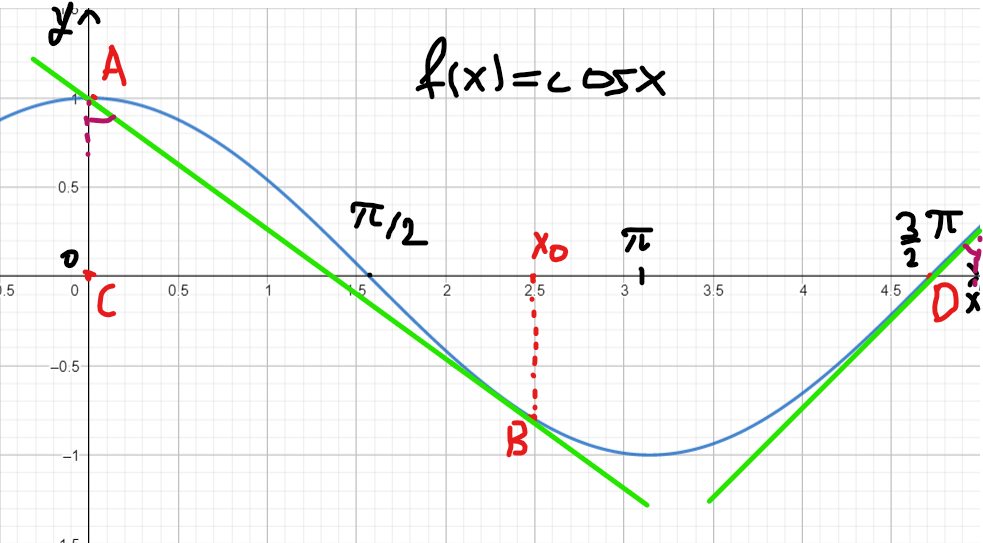
\includegraphics[scale=0.7]{pictures/task_07_01.png}
\end{center}

\underline{\textbf{Answer:}}
$
    \partial f(x) = \begin{cases}
        [-\infty, -sinx], x = 0 \\
        \varnothing, x \in (0, x_0) \\
        -sinx, x \in [x_0, \frac{3}{2} \pi) \\
        [1, +\infty], x = \frac{3}{2} \pi
    \end{cases}
$

\subsection{Problem №3}
Find $\partial f(x)$, if $f(x) = ||Ax - b||_1^2$

\underline{\textbf{Solution:}}
By property of subdifferential we can get 
that:
\begin{equation*}
\partial(||Ax - b||_1^2) = ||Ax - b||_1 \partial(||Ax-b||_1)     
\end{equation*}
From the seminar we know that:
\begin{equation*}
    \partial||y||_1 = \{\alpha : ||\alpha||_{\infty} \leq 1, \alpha^Ty = ||y||_1\}
\end{equation*}
And now we can get that (by another property of subdifferential:
\begin{equation*}
    \partial\left(||Ax - b||_1^2 \right) = ||Ax - b||_1 \partial \left(||Ax-b||_1 \right)(x) = ||Ax - b||_1A^T \partial ||Ax+b||_1
\end{equation*}


\begin{equation*}
 ||Ax - b||_1A^T \partial ||Ax+b||_1 = ||Ax - b||_1A^T \cdot \{\alpha : ||\alpha||_{\infty} \leq 1, \alpha^T (Ax+b ) = ||Ax+b||_1\}
\end{equation*}

\underline{\textbf{Answer:}} $\partial f(x) = ||Ax - b||_1A^T \cdot \{\alpha : ||\alpha||_{\infty} \leq 1$, $\alpha^T (Ax+b ) = ||Ax+b||_1\}$

\subsection{Problem №4}
Suppose, that if $f(x) = ||x||_{\infty}$. Prove that $\partial f(0) = $ \textbf{conv} $\{\pm e_1, ..., \pm e_n \}$, where $e_i$ is i-th canonical basis vector (column of identity matrix).

\underline{\textbf{Solution:}}
By the definition: $f(x) = ||x||_{\infty} = \max\limits_i |x_i|$

We know that subbdifferential for module is equal:
\begin{equation*}
    \partial |x_i| = \begin{cases} 
    x_i, x_i > 0\\
    [-1, 1], x_i = 0 \\
    -x_i, x_i < 0
    \end{cases}
\end{equation*}

Because $|x_i|$ -- convex functions, by Dubovitsky - Milutin theorem we can get:
\begin{equation*}
    \partial f(0) = conv \left\{ \bigcup\limits_{i \in \overline{1, n}} \partial|x_i|_{x_i = 0} \right\} = conv \left\{\pm e_1, ..., \pm e_n\right\}\text{, } e_i \text{ is i-th canonical basis vector}
\end{equation*}

WOHOO, we proved that!

\subsection{Problem №5}
Find $\partial f(x)$, if $f(x) = e^{||x||}$. \\Try do the task for an arbitrary norm. At least, try $||\cdot || = ||\cdot||_{\{2, 1, \infty \}}$

\underline{\textbf{Solution:}}
\newline
By the property of subdifferential we: $\partial f(x) = \partial(e^{||x||}) = e^{||x||} \partial(||x||)$
\newline
And now we need to find $\partial ||x||$ for $||x||_1, ||x||_2$ and $||x||_{\infty}$
\newline
\textbf{1.}
In the seminar we find that and it equals: 
\begin{equation*}
\partial||x||_1 = \{\alpha : ||\alpha||_{\infty} \leq 1, \alpha^Tx = ||x||_1\}
\end{equation*}
\newline
\textbf{2.}
By definition $||x||_2 = \sqrt{\sum\limits_{i = 1}^n x_i^2}$, this function is differentiable everywhere except zero. 
\newline
For $x \not = 0$, $\partial f(x) = \nabla ||x||_2 =\frac{x}{||x||_2}$
\newline
Now we need to consider $x = 0$: let's find such interesting limit: $\lim\limits_{\beta \xrightarrow{} 0+} \frac{||\beta e||_2}{\beta} = ||e||_2$, where e is unit vector on unit sphere.

But by definition $\frac{x}{||x||_2} = e$,  and we get that 
\begin{equation*}
\partial ||x||_2 = \{e \text{ | } ||e||_2 \leq 1 \}    
\end{equation*}
\newline
\textbf{3.}
In \underline{problem №4} I find that ($x_i$ - maximum element by modules):
\begin{equation*}
    ||x||_{\infty} = \begin{cases}
            [-1, 1], \text{ if } i x_i = 0 \\
            sign(x_i), x_i \not = 0
    \end{cases}
\end{equation*}

\underline{\textbf{Answer:}}

\begin{itemize}
    \item for $|| \cdot ||_1$: $\partial f(x) = e^{||x||_1} \cdot \{\alpha : ||\alpha||_{\infty} \leq 1, \alpha^Tx = ||x||_1\}$
    \item for $|| \cdot ||_2$: $\partial f(x) = e^{||x||_2} \cdot \{e \text{ | } ||e||_2 \leq 1 \}$
    \item for $|| \cdot ||_{\infty}$: $\partial f(x) = e^{||x||_{\infty}} \cdot \begin{cases}
            [-1, 1], \text{ if } x_i = 0 \\
            sign(x_i), x_i \not = 0
    \end{cases}$, where is $x_i$ -- maximum element by modules
\end{itemize}


